%!TEX program = lualatex
%!TEX encoding = UTF-8 Unicode  
%!TEX root = chapter07.tex  
\documentclass[main.tex]{subfiles} 
\begin{document} 
%----------------------------------------------------------------------------------------
%	CHAPTER 7
%----------------------------------------------------------------------------------------
\cleardoublepage 
\loadgeometry{marginlayout}  
\pagestyle{scrheadings} % Print headers again  
\KOMAoptions{
headwidth=textwithmarginpar,
headsepline=true,
headsepline= 0.5pt,
footwidth=textwithmarginpar,
}   
\onehalfspacing 
\setcounter{chapter}{6}
\chapter{Généralités sur les fonctions}



\section{Définition}
\textbf{Un couple}  de 2 nombres $x$ et $y$ se note $(x,y)$ (parenthèses et une virgule pour séparer ses deux composants). \\
Le 1\ier nombre $x$ s'appelle l'\textbf{abscisse}. Le 2\up{nd} $y$ s'appelle l'\textbf{ordonnée}.  
\begin{definition}[fonction identifiée à son graphe] 
	Une fonction $f$ est un \textbf{ensemble de couples} $(x,y)$, tel qu'il n'y ait pas 2 couples  ayant la même abscisse mais des ordonnées différentes.  \\
	Pour un couple $(x,y)$ de la fonction, on dit :
	\begin{enumerate}[label=\textbullet,leftmargin=*]
		\item \og \textbf{ordonnée $y$ est l'image de l'abscisse $x$} \fg{}  
		\item \og \textbf{l'abscisse $x$ est un antécédent de l'ordonnée $y$} \fg{}.  
	\end{enumerate} 
\end{definition} 

\begin{description}
	\item[Notation 1] \og $f\colon x\mapsto y$ \fg \quad à lire \og	$f$ associe à la valeur $x$ l'ordonnée $y$ \fg{}
	\item[Notation 2] \og $y = f(x)$ \fg \quad  à lire \og y égal à $f$ de $x$ \fg{}, notation due à Euler vers 1850 
\end{description}  
%%%%%%%%%%%%%%%%%%%%%%%%%%%%%%%%%%%%%%%%%%%%%%%%%%%%%%%%%%%
%
%%%%%%%%%%%%%%%%%%%%%%%%%%%%%%%%%%%%%%%%%%%%%%%%%%%%%%%%%%% 
\newpage 
\section{Représentations de fonctions}
\subsection{Par un tableau de valeurs} 
On peut représenter l'ensemble des couples $(x,y)$ d'une fonction par un tableau de valeurs en ligne ou en colonne.
\begin{table}[h]
	$$\def\arraystretch{1.5}\begin{array}{|l|c|c|c|c|c|}
		\hline
		x & 12 & 17 & -5 & -1 & 9 \\
		\hline
		f(x) & -1 & 9 & 18 & -5 & -1 \\
		\hline
	\end{array}
	$$
	\caption{L'image de $-5$ par $f$ est $18$ : $f(-5)=18$}
\end{table}
\subsection{Par une représentation représentative} 
La représentation graphique d'une fonction $f$ est l'ensemble des points du plan $M(x;y)$ dont le couple de coordonnées vérifient $y=f(x)$  ( l'ordonnée de $M$ est l'image de l'abscisse de $M$ par $f$). 
\begin{figure}[h]\centering
	\begin{tikzpicture}[xscale=1.0, yscale=1]
		\tkzSetUpPoint[size=3, fill=black]
		\tkzfctset{tan style/.style={->,>=latex, color=red, line width=1.2pt}}  
		\tkzInit[xmin=-6.0,xmax=5.0,ymin=-3.0,ymax=6.5,xstep=1.0, ystep=1.0]; 
		\tkzFct[domain = -5.5:6,  line width=1.0pt]{ 
			.1*(\x+5)*(\x+2)*(3.25-\x)*exp(\x/6)-1	+ (\x+5)*(\x+2)/(4.2*1.2)*0.214
		}; 
		\tkzDefPointByFct[ref=P]({-2});
		\tkzDefPointByFct[ref=P4]({-5});
		\tkzDrawPoint[ color=black, size=5, fill=black, shape=cross ](P4) 
		\tkzDrawX[   color=blue, line width=1.2pt];
		\tkzDrawY[  color=red, line width=1.2pt] ;
		\tkzText[below right](0,0){O}; 
		\tkzText[below ](1,0){1}; 
		\tkzText[right](0,1){1};
		\tkzDefPointByFct[ref=P2]({-3.5}) 
		% 		\draw  [very thick, -{Arc Barb[reversed]}] (P4)  --++ (-0.1,0) ;
		% 		\tkzDefPointByFct[ref=P5]({3}) 
		% 		\tkzDrawPoint[color=black, size=4, fill=black](P5);
		\tkzPointShowCoord[ xlabel={}, xstyle={above=6pt} ](P2)
		\tkzDrawPoint[ color=black, size=5, fill=black, shape=cross ](P) 
		\tkzPointShowCoord(P4)  
		\tkzDefPointByFct[ref=P3]({2.385}) 
		\tkzPointShowCoord[   xlabel={\color{blue}$x$}, xstyle={below=6pt} , ylabel={\color{red}$y=f(x)$}, ystyle={left} ](P3)
		\tkzLabelPoint[right](P3){\small$M(x;y)$}	
		\tkzDefPoint(-4.5,-2.5){T1} 
		\tkzText[color = black, above, fill=white](T1){$\mathscr{C}_f$}
		\tkzDefPoint(4.0,-1.5){A1}
		\tkzDefPoint(4.5,0){A2}
		\tkzDefPoint(2.385,3.4){Q1}
		\tkzDefPoint(2.385,5.8){Q2}
		\tkzPointShowCoord[noydraw](P)  	
		\tkzLabelPoint[below right](P){\small$A($}	
		\tkzLabelPoint[below right](P2){\small$B($}
		% 	 		\tkzLabelPoint[below](P2){\small$B$}
		\tkzPointShowCoord[  ylabel={\color{red}$y'\neq f(x)$}, xstyle={below=6pt}](Q2)
		% 	 		 		\tkzPointShowCoord[noxdraw, ylabel={\color{red}$y"$},xstyle={below=6pt}](Q1)
		\tkzLabelPoint[right](Q2){\scriptsize$N(x;y')$ n'appartient pas à $\mathscr{C}_f$} 
		\draw[->,>=latex] (A1) to[bend right=15] (A2);
		\tkzText[color = black, below, fill=white,text width=3.8cm](A1){Axe des abscisses, où lire les antécédents}
		\tkzDefPoint(-2.1,6.3){A3}
		\tkzDefPoint(0,6.4){A4}
		\draw[->,>=latex] (A3) to[bend left=15] (A4);
		\tkzText[color = black, left, fill=white,text width=3.5cm](A3){Axe des ordonnées où lire l'image}	
	\end{tikzpicture}
	\caption{La représentation graphique d'une fonction ne peut pas avoir deux points ayant même abscisse et des ordonnées différentes.}
\end{figure}
%%%%%%%%%%%%%%%%%%%%%%%%%%%%%%%%%%%%%%%%%%%%%%%%%%%%%%%%%%%
%
%%%%%%%%%%%%%%%%%%%%%%%%%%%%%%%%%%%%%%%%%%%%%%%%%%%%%%%%%%% 
\newpage 
\section{Expressions algébriques de fonctions}
Certaines fonctions, se présentent comme un programme de calcul qui permet d'obtenir la valeur de l'ordonnée $y$ lorsque l'on connait la valeur de l'abscisse $x$. Souvent il s'agit d'une expression algébrique de la variable $x$. 
\begin{example}Soit $f$ la fonction définie par l'expression  :
	$$f\colon x\mapsto x^2\qquad f(x)=x^2$$ 
	\begin{align*}
		f&\colon 3 \mapsto 3^2 =9 \\
		f(3)& = 3^2=9 && \text{l'image de $3$ par $f$ est $9$}\\ 
		f&\colon 5 \mapsto 5^2 =9 \\
		f(5)& = 5^2=25 && \text{l'image de $5$ par $f$ est $25$}\\ 
		f&\colon -4 \mapsto (-4)^2 =16 \\
		f(-4)& = (-4)^2=16 && \text{l'image de $-4$ par $f$ est $16$} 
	\end{align*}
\end{example}
\begin{example} Soit la fonction $f : x\mapsto 3x+1 $. Pour calculer l'image de $2$ par la  $f$ on fait $$f(2)=3\times 2 +1=7$$  
\end{example}
\begin{example}
	Soit la fonction $g$ définie par $g(x)=x^2-3x+2$. 
	L'image de $-1$ vaut 
	$$g(-1)=(-1)^2-3\times(-1)+2 =6$$
\end{example}
 
%----------------------------------------------------------------------------------------
%	EXERCICES
%----------------------------------------------------------------------------------------

\newpage 
\loadgeometry{widelayout}  
\pagestyle{scrheadings} % Print headers again  
\KOMAoptions{
	headwidth=textwithmarginpar,
	headsepline=true,
	headsepline= 0.5pt,
	footwidth=textwithmarginpar,
} 
\onehalfspacing
\section{Exercices}
\begin{example}[fonction par son graphe]\hfill \\
	Soit les ensembles de couples ordonnés suivant :
	\begin{multicols}{2} 
		\begin{description}  
			\item[$f=$]  $\left\{ {\left( {6,10} \right),\left( { - 7,3} \right),\left( {0,4} \right),\left( {6, - 4} \right)} \right\}$  
			\item[$g=$]  $\left\{ {\left( { - 1,0} \right),\left( {0, - 3} \right),\left( {2, - 3} \right),\left( {3,0} \right),\left( {4,5} \right)} \right\}$ 
		\end{description}
	\end{multicols}
	\begin{enumerate}
		\item Le couple ordonné $(6;10)$ de $f$ est représenté par une flèche partant de $6$ et pointant vers $10$. Compléter les graphes orientés ci-dessous pour représenter les ensembles $f$ et $g$.    \\
		
		\begin{minipage}{0.5\columnwidth}
			
			%			\begin{figure}[h]{1\columnwidth}\centering
			% Define layers
			\pgfdeclarelayer{background}
			\pgfdeclarelayer{foreground}
			\pgfsetlayers{background,main,foreground}
			\begin{tikzpicture}[
				> = latex, % arrow head style
				shorten > = 1pt, % don't touch arrow head to node
				auto,
				node distance =1.50em, % distance between nodes
				semithick % line style
				]
				
				\tikzstyle{every state}=[
				%        draw = black, 
				draw=none,
				%        thick,
				%        fill = white,
				minimum size = 4mm
				]
				\node[state] (x1){$-7$};
				\node[state] [above of=x1] (x0){Abscisses};
				\node[state] [below of=x1] (x2){$0$}; 
				\node[state] [below of=x2] (x3){$1$}; 
				\node[state] [below of=x3] (x4){$2$}; 
				\node[state] [below of=x4] (x5){$6$};
				
				
				\node[state] [right of=x1, xshift=2cm, yshift=1em] (y1){$10$};
				
				\node[state] [above of=y1] (y0){Ordonnées};
				\node[state] [below of=y1] (y2){$3$};
				\node[state] [below of=y2] (y3){$4$} ;
				\node[state] [below of=y3] (y4){$-1$} ;
				\node[state] [below of=y4] (y5){$-4$} ;
				
				%     \path[|->] (x1) edge (y2);
				%     \path[|->] (x2) edge (y3);
				%     \path[|->] (x3) edge (y1);
				\path[|->] (x5) edge  (y1);
				%     \path[|->] (x5) edge (y5);
				%\path[->] (x5) edge node {} (y3);
				
				%    \draw[red, dashed] (1, 2) -- (1, -2);
				\begin{pgfonlayer}{background}
					\draw[rounded corners=2em,line width=3em,blue!20,cap=round]
					(x1.north) -- (x2.center) -- (x3.center)--  (x5.south);
					\draw[rounded corners=2em,line width=3em,red!20,cap=round]
					(y1.north) -- (y2.center) -- (y3.center) -- (y5.south);
				\end{pgfonlayer}
			\end{tikzpicture} 
			%				\caption{graphe orienté pour représenter $f$}
			%			\end{figure} 
		\end{minipage} 
		\begin{minipage}{0.5\columnwidth} 
			%			\begin{figure}{1\columnwidth}\centering
			% Define layers
			\pgfdeclarelayer{background}
			\pgfdeclarelayer{foreground}
			\pgfsetlayers{background,main,foreground}
			\begin{tikzpicture}[
				> = latex, % arrow head style
				shorten > = 1pt, % don't touch arrow head to node
				auto,
				node distance = 1.50em, % distance between nodes
				semithick % line style
				]
				
				\tikzstyle{every state}=[
				%        draw = black, 
				draw=none,
				%        thick,
				%        fill = white,
				minimum size = 4mm
				]
				\node[state] (x1){$-1$};
				\node[state] [below of=x1] (x2){$0$};
				\node[state] [below of=x2] (x3){$2$};
				\node[state] [below of=x3] (x4){$3$};
				\node[state] [below of=x4] (x5){$4$};
				\node[state] [above of=x1] (x6){$-2$};
				\node[state] [above of=x6] (x0){Abscisses};
				
				
				\node[state] [right of=x2, xshift=2cm, yshift=1em] (y1){$-3$};
				\node[state] [above of=y1] (y0){Ordonnées};
				\node[state] [below of=y1] (z2){$-1$};
				\node[state] [below of=z2] (y2){$0$};
				\node[state] [below of=y2] (y3){$5$} ;
				
				\path[|->] (x1) edge (y2);
				%           \path[|->] (x2) edge (y1);
				%           \path[|->] (x3) edge (y1);
				%           \path[|->] (x4) edge  (y2);
				%           \path[|->] (x5) edge (y3);
				%\path[->] (x5) edge node {} (y3);
				
				%    \draw[red, dashed] (1, 2) -- (1, -2);
				\begin{pgfonlayer}{background}
					\draw[rounded corners=2em,line width=3em,blue!20,cap=round]
					(x6.north) -- (x2.center) -- (x3.center)-- (x4.center)-- (x5.south);
					\draw[rounded corners=2em,line width=3em,red!20,cap=round]
					(y1.north) -- (y2.center) -- (y3.south);
				\end{pgfonlayer}
			\end{tikzpicture}
			%				\caption{graphe orienté pour  $g$}
			%			\end{figure} 
		\end{minipage} 
		\item  \begin{multicols}{2}
			$f$ n'est pas une fonction   
			
			$g$ est une fonction.
		\end{multicols}
		\vfill 
		\item Compléter les pointillés : 
		\begin{enumerate}
			\item    $g\colon \ldots \mapsto 0$. \hfill $g\colon \ldots \mapsto 0$.\hfill $g\colon \ldots \mapsto -3$. \hfill $g\colon \ldots \mapsto -3$. \hfill $g\colon 4 \mapsto \ldots $.
			\item $g(3) = \ldots$.\hfill $g(\ldots)=0$. \hfill $5=g(\ldots)$.\hfill $\ldots=g(0)$. \hfill $-1=g(\ldots)$.
			\item $-3$ est \dotfill de $0$ par $g$.\hfill $0$ a pour \dotfill $-3$  par $g$.
			\item $-1$ est   \dotfill  de $0$  par $g$.\hfill $-1$ a pour \dotfill $0$  par $g$
			\item Les nombres \dotfill ont pour image $0$ par $g$.
			\item Les antécédents de $-3$ par $g$ sont \dotfill 
		\end{enumerate} 
	\end{enumerate} 
\end{example}
\begin{example}[fonction par son tableau de valeurs]\hfill 
	
	Voici un tableau de valeurs d'une fonction $f$ :  
	$$\def\arraystretch{1.5}\begin{array}{|l|c|c|c|c|c|}
		\hline
		x & 19 & -15 & 8 & -3 & 9 \\
		\hline
		y=f(x) & -15 & -2 & 19 & 19 & 8 \\
		\hline
	\end{array}
	$$
	\begin{enumerate}
		\item Quelle est l'image de $-15$ par la fonction $f$ ?
		\item Quelle est l'image de $8$ par la fonction $f$ ?
		\item Déterminer le(s) antécédent(s) de $-15$ par la fonction $f$.
		\item Déterminer le(s) antécédent(s) de $19$ par la fonction $f$.
		\item Compléter : $f(8)=\ldots$
		\item Compléter : $f(\ldots)=8$
	\end{enumerate}
\end{example}

\begin{example}[fonction par sa représentation graphique]  
	On désire mesurer tout au long d'une journée la température extérieure en fonction du temps.	Voici la courbe obtenue au bout de 24h consécutives. 
	
	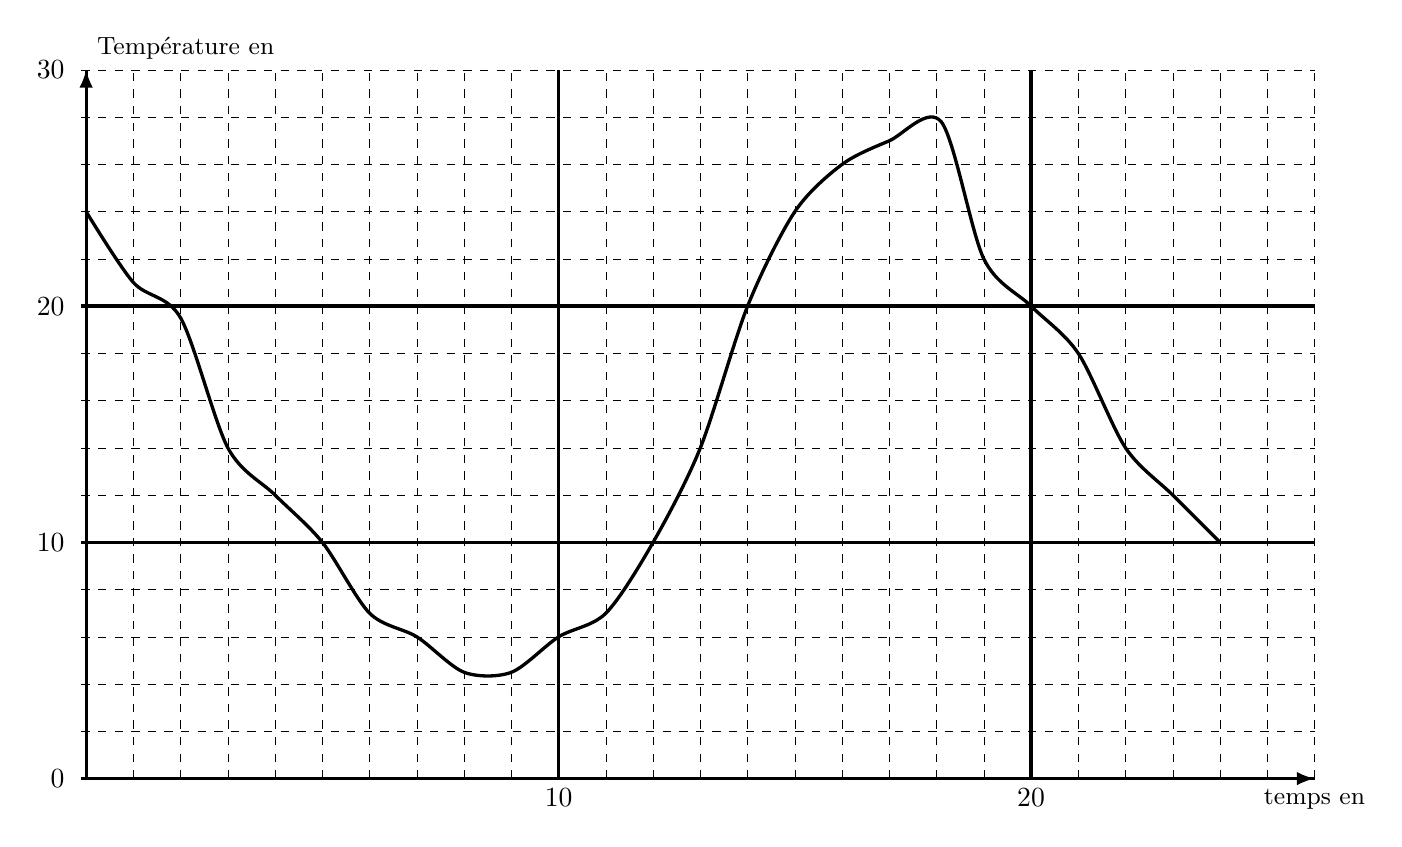
\begin{tikzpicture}[xscale=0.6, yscale=0.3]
		\tkzInit[xmin=0,xmax=26,ymin=0,ymax=30,xstep=1.0, ystep=1.0];
		\begin{scope}[dashed]
			\tkzGrid(0, 0)(26.0,30.0); 
			%	[ sub,color=gray,subcolor=gray!20,subxstep=1.0,subystep=2.0] 
			\draw [ very thin] (-0.1,0) grid[xstep=1,ystep=2] (26,30);
		\end{scope}
		\draw [ very thick](-0.1,0) grid[xstep=10,ystep=10] (26,20);
		\draw [ very thick](-0.1,0) grid[xstep=10,ystep=50] (20,30);
		\draw[very thick , black ] plot[smooth] coordinates {(0,24)(1,21)(2,19.5)(3,14)(4,12)(5,10)(6,7)(7,6)(8,4.5)(9,4.5)(10,6)(11,7)(12,10)(13,14)(14,20)(15,24)(16,26)(17,27)(18.1,27.8)(19,22)(20,20)(21,18)(22,14)(23,12)(24,10)};
		\draw[->,>=latex,very thick] (0,0)--(26,0) node[below]{\small{temps en \si{\hour}}};
		\draw[->,>=latex,very thick] (0,0)--(0,30) node[above right]{\small{Température en \si{\celsius}}};
		\foreach \x in {10,20} \draw (\x,0) node[below]{\x};
		\foreach \y in {0,10,20,30} \draw (-0.25,\y) node[left]{\y};
	\end{tikzpicture}
	\begin{mdframed} 
		La courbe n'a pas de points qui ont la même abscisse mais des ordonnées différentes. \\
		On dit que la température $T$ (l'ordonnée) est une \textbf{fonction} de l'heure $h$ (l'abscisse).
	\end{mdframed}
	\begin{enumerate}
		\item Quelle grandeur est représentée sur l'axe des abscisses ?\dotfill
		\item Quelle grandeur est représentée sur l'axe des ordonnées ?\dotfill   
		\item \begin{enumerate}
			\item Donner l'ordonnée d'un point de la courbe d'abscisse 10 et interpréter le résultat par une phrase. Y a-t'il plusieurs réponses possibles ?
			\item Donner l'ordonnée \textbf{du} point de la courbe d'abscisse 14 et interpréter le résultat. 
		\end{enumerate} 
		
		%		On note \og $T(h)$ \fg{} \textbf{la} température à l'heure $h$. Si $h=10$, alors $T(10)$ est la température à l'heure $10$.
		%		
		%		Les écritures suivantes sont synonymes :\\
		%		\og 10 a pour image 6 par la fonction $T$\fg{} revient à \og  $T\colon 10 \mapsto 6$ \fg{} revient à  \og $T(10)=6$ \fg{}. 
		
		\item Compléter les pointillés :
		\begin{enumerate}[label=\textbullet]
			\item \og 12 a pour image $\ldots$ par la fonction $T$ \fg{} \og $T\colon 12 \mapsto \ldots $ \fg{} \og $T(12)=\ldots$\fg{}
			\item \og $\ldots$ a pour image $\ldots$ par la fonction $T$ \fg{} \og $T\colon 3 \mapsto \ldots $ \fg{} \og $T(\ldots)=\ldots$\fg{}
			\item \og $\ldots$ a pour image $\ldots$ par la fonction $T$ \fg{} \og $T\colon \ldots \mapsto \ldots $ \fg{} \og $T(5)=\ldots$\fg{}
		\end{enumerate}
		\item \begin{enumerate}
			\item À quelle(s) heure(s) la température était-elle de $\SI{14}{\celsius}$ ? \dotfill 
			\item Répondre à la question précédente en complétant :\\
			$T(\ldots)=\ldots$ \hfill $T(\ldots)=\ldots$ \hfill $T(\ldots)=\ldots$ \hfill \null $T(\ldots)=\ldots$ \hfill \null
			\item À quelle(s) heure(s) la température était-elle de $\SI{10}{\celsius}$ ? Répondre en complétant les pointillés avec la précision permise par le graphique.\\
			$T(\ldots)=\ldots$ \hfill $T(\ldots)=\ldots$ \hfill $T(\ldots)=\ldots$ \hfill \null $T(\ldots)=\ldots$ \hfill \null
			\item  À quelle(s) heure(s) la température était-elle de $\SI{23}{\celsius}$ ? \\
			$T(\ldots)=\ldots$ \hfill $T(\ldots)=\ldots$ \hfill $T(\ldots)=\ldots$ \hfill \null $T(\ldots)=\ldots$ \hfill \null
			\item  À quelle(s) heure(s) la température était-elle de $\SI{28}{\celsius}$ ? \\
			$T(\ldots)=\ldots$ \hfill $T(\ldots)=\ldots$ \hfill $T(\ldots)=\ldots$ \hfill \null $T(\ldots)=\ldots$ \hfill \null
			\item  À quelle(s) heure(s) la température était-elle de $\SI{30}{\celsius}$ ? \\
			$T(\ldots)=\ldots$ \hfill $T(\ldots)=\ldots$ \hfill $T(\ldots)=\ldots$ \hfill \null $T(\ldots)=\ldots$ \hfill \null
		\end{enumerate}
		%		\begin{mdframed}
		%			On a vu que \og 6 est l'image de 10\fg{}. On peut dire \og  6 est \textbf{un} antécédent de 10 \fg{}. 
		%			
		%			Une abscisse a une   unique image par une fonction.\\
		%			Par contre une ordonnée peut avoir aucun, un  ou plusieurs antécédents.
		%		\end{mdframed}
		\item On peut représenter certains couples (abscisse, ordonnée) à l'aide d'un tableau de valeurs. Compléter le tableau suivant :
		
		\begin{minipage}{1\columnwidth}\centering
			\begin{tabularx}{0.95\columnwidth}{|c?X|X|X|X|X|X|X|X|X|X|X|X|X|X|}\hline 
				$x$		&0	& & 6& 	 &	10   &	 	& 18 & 		&	18,1 & 		& 	&  &&\\ \hline 
				$T(x)$	& 	&6&	 & 10&		 &10	& 	 &  19	&27,8& 27,8	& 16 &	20	&20 & 20\\ \hline 
			\end{tabularx}
			%			\begin{enumerate}
			%				\item Pouvez vous donner un avantage de l'utilisation d'une représentation graphique à celle d'un tableau ?\dotfill \\
			%				\null \dotfill\null
			%				\item Pouvez vous donner un avantage de l'utilisation d'un tableau de valeurs à celle d'une représentation graphique ?\dotfill \\
			%				\null \dotfill\null
			%			\end{enumerate}
		\end{minipage}
		%	\\
	\end{enumerate}
	%	\faWarning~ Un tableau de valeurs n'est pas forcément un tableau de proportionnalité !
\end{example}

\begin{example}[fonction définie par un programme de calcul ou une expression]\hfill  
	\begin{enumerate}
		\item On donne le programme de calcul suivant qui correspond à une certaine fonction :
		
		\noindent\fbox{\parbox{0.5\linewidth}{
				\begin{itemize}
					\item Choisir un nombre
					\item Multiplier ce nombre par 5
					\item Ajouter 9 au résultat obtenu
				\end{itemize}
			}
		} 	 
		\begin{enumerate}
			\item Appliquer ce programme de calcul au nombre 3
			\item Traduire ce calcul par une phrase contenant le mot image
		\end{enumerate}
		
		\item Soit $f$ la fonction définie par l'expression algébrique $f(x)=$ 5$x+$9\begin{enumerate}
			\item Calculer l'image de 2
			\item Traduire ce calcul par une phrase contenant le mot image
		\end{enumerate}
		
		\item Soit $g$ la fonction définie par $g:x\longmapsto \frac{5}{6x+2}$  \begin{enumerate}
			\item Calculer l'image de 9
			\item Traduire ce calcul par une phrase contenant le mot image
		\end{enumerate}
		
		\item Soit la fonction $h$ définie par le diagramme \\
		
		\definecolor{frvzsz}{rgb}{0.9450980392156862,0.34901960784313724,0.1607843137254902}
		\begin{tikzpicture}[line cap=round,line join=round,>=triangle 45,x=1cm,y=1cm]
			\draw [line width=3pt,color=frvzsz] (-10,0.5) -- (-9,0.5) -- (-9,-0.5) -- (-10,-0.5) -- cycle;
			\node[text width=3cm,text centered, scale=1] at(-9.5,0){$x$};
			
			\draw [line width=3pt,color=frvzsz] (-9,0) -- (-8.5,0);
			\draw [line width=3pt,color=frvzsz] (-8,0) circle(0.5);
			\node [text width=3cm,text centered, scale=1] at(-8,0){$\times 7$};
			\draw [->,line width=3pt,color=frvzsz] (-7.5,0) -- (-6.5,0);
			\draw [line width=3pt,color=frvzsz] (-6.5,0.5) -- (-5.5,0.5) -- (-5.5,-0.5) -- (-6.5,-0.5) -- cycle;
			\node [text width=3cm,text centered, scale=1] at(-6,0){$7x$};
			
			\draw [line width=3pt,color=frvzsz] (-5.5,0) -- (-5,0);
			\draw [line width=3pt,color=frvzsz] (-4.5,0) circle(0.5);
			\node [text width=3cm,text centered, scale=1] at(-4.5,0){$+8$};
			\draw [->,line width=3pt,color=frvzsz] (-4,0) -- (-3,0);
			\draw [line width=3pt,color=frvzsz] (-3,0.5) -- (0,0.5) -- (0,-0.5) -- (-3,-0.5) -- cycle;
			\node [text width=3cm,text centered, scale=1] at(-1.5,0){$h(x)=7x+8$};
			
		\end{tikzpicture}
		\begin{enumerate}
			\item Calculer $h(7)$
			\item Traduire ce calcul par une phrase contenant le mot image
		\end{enumerate} 
		\item Soit la fonction $i$ définie par le diagramme \\ \definecolor{frvzsz}{rgb}{0.9450980392156862,0.34901960784313724,0.1607843137254902}
		\begin{tikzpicture}[line cap=round,line join=round,>=triangle 45,x=1cm,y=1cm]
			\draw [line width=3pt,color=frvzsz] (-10,0.5) -- (-9,0.5) -- (-9,-0.5) -- (-10,-0.5) -- cycle;
			\node[text width=3cm,text centered, scale=1] at(-9.5,0){$x$};
			
			\draw [line width=3pt,color=frvzsz] (-9,0) -- (-8.5,0);
			\draw [line width=3pt,color=frvzsz] (-8,0) circle(0.5);
			\node [text width=3cm,text centered, scale=1] at(-8,0){$- 2$};
			\draw [->,line width=3pt,color=frvzsz] (-7.5,0) -- (-6.5,0);
			\draw [line width=3pt,color=frvzsz] (-6.5,0.5) -- (-5.5,0.5) -- (-5.5,-0.5) -- (-6.5,-0.5) -- cycle;
			\node [text width=3cm,text centered, scale=1] at(-6,0){$ \qquad $};
			
			\draw [line width=3pt,color=frvzsz] (-5.5,0) -- (-5,0);
			\draw [line width=3pt,color=frvzsz] (-4.5,0) circle(0.5);
			\node [text width=3cm,text centered, scale=1] at(-4.5,0){$\times 5$};
			\draw [->,line width=3pt,color=frvzsz] (-4,0) -- (-3,0);
			\draw [line width=3pt,color=frvzsz] (-3,0.5) -- (0,0.5) -- (0,-0.5) -- (-3,-0.5) -- cycle;
			\node [text width=3cm,text centered, scale=1] at(-1.5,0){$i(x)=\qquad\qquad$};
			
		\end{tikzpicture}
		\begin{enumerate}
			\item Exprimer l'image $i(x)$ en fonction de $x$ sous forme développée réduite.
			\item Calculer  $i(-3)$
			\item Traduire ce calcul par une phrase contenant le mot image
		\end{enumerate} 
	\end{enumerate}
\end{example}

%%%%%%%%%%%%%%%%%%%%%%%%%%%%%%%%%%%%%%%%%%%%%%%%%%%%%%%%%%%
%
%%%%%%%%%%%%%%%%%%%%%%%%%%%%%%%%%%%%%%%%%%%%%%%%%%%%%%%%%%%
\newpage  
%\begin{exercise}\hfill
%	
%	Écrire l'expression de la fonction $f$ à partir de son programme de calculs :
%	\begin{enumerate}[leftmargin=*]
%%		\setcounter{enumi}{9}
%		\item $f$ est la fonction qui, à un nombre, associe  son opposé.  
%		$f(x) = $ \dotfill 
%		\item $g$ est la fonction qui, à un nombre, associe le double de son inverse.  
%		$g(x) = $ \dotfill 
%		\item $h$ est la fonction qui, à un nombre, associe la somme des trois-quarts de ce nombre et de $-5$. \\
%		$h(x) = $ \dotfill 
%		\item $i$ est la fonction qui, à un nombre, associe le carré de la somme de ce nombre et de $\sqrt{5}$ . 	\\ 
%		$i(x) = $ \dotfill 
%		\item  $j$ est la fonction qui, à un nombre, associe le quotient de son cube par 9. \\
%		$j(x) = $\dotfill 
%	\end{enumerate}
%\end{exercise}
\begin{exercise}\hfill
	
	Soit la fonction $f$ représentée par le tableau de valeur suivant :\\
	\begin{minipage}{1\columnwidth}\centering
		\begin{tabular}{|c?c|c|c|c|c|c|c|c|c|c|}\hline 
			$x$	&0	&- 1&	4&	5&	2	&- 2	& 8	&3	&- 5&	1 \\ \hline 
			$f(x)$	&- 4	&0	&0	&8	&6	&- 6	&5	&14&	6	&- 6\\ \hline
		\end{tabular}
	\end{minipage}\\
	Pour chaque question vous répondrez en précisant l'égalité $f(\ldots)=\ldots$ correspondante.
	\begin{enumerate}[leftmargin=*]
		% 	\setcounter{enumi}{12}
		\item Donner un antécédent de $8$.\dotfill 
		\item Quelle est l'image  de $0$?\dotfill 
		\item Quelle est l'image de $4$?\dotfill 
		\item Donner un antécédent de $14$.\dotfill 
		\item Y a-t-il un nombre du tableau égal à son image?\dotfill 
		\item Citer des valeurs de  $x$  telles que  $f(x) = - 6$.\dotfill 
		\item Citer un nombre strictement négatif ayant un antécédent strictement positif.\dotfill 
		\item Citer deux nombres opposés dont les images sont des nombres opposés.\dotfill 
		\item Trouver deux nombres $a$ et $b$ image l'un de l'autre pas $f$.\dotfill 
	\end{enumerate} 
\end{exercise} 
\begin{exercise}\hfill 
	\begin{enumerate}
		\item On considère la fonction $f$ définie par $f:x\mapsto -11x^2-3x$. Calculer $f(-1)$.
		\item On considère la fonction $g$ définie par $g:x\mapsto 4x^2+3x+7$. Calculer $g(3)$.
		\item On considère la fonction $h$ définie par $h:x\mapsto (-2x+3)^2$. Calculer $h(1)$.
		\item On considère la fonction $i$ définie par $i:x\mapsto -5x^2+9x-11$. Calculer $i(12)$.
		\item On considère la fonction $j$ définie par $j:x\mapsto \dfrac{7x+7}{3x+8}$. Calculer $j(-12)$.
	\end{enumerate}
\end{exercise}
\begin{exercise}\hfill 
	\begin{multicols}{2}
		\begin{enumerate}[leftmargin=*]
			\item On considère la fonction $f$ définie par $f:x\mapsto 4x^2-2$. Compléter le tableau de valeurs suivant.
			
			\medskip
			$\begin{array}{|l|c|c|c|}
				\hline
				x & -2 & 0 & 2 \\
				\hline
				f(x) & \phantom{-10} & \phantom{-10} & \phantom{-10} \\
				\hline
			\end{array}
			$
			\item On considère la fonction $g$ définie par $g:x\mapsto 2x^2+8$. Compléter le tableau de valeurs suivant.
			
			\medskip
			$\begin{array}{|l|c|c|c|}
				\hline
				x & 1 & 2 & 5 \\
				\hline
				g(x) & \phantom{-10} & \phantom{-10} & \phantom{-10} \\
				\hline
			\end{array}
			$
			\item On considère la fonction $h$ définie par $h:x\mapsto 9x$. Compléter le tableau de valeurs suivant.
			
			\medskip
			$\begin{array}{|l|c|c|c|}
				\hline
				x & -3 & 6 & 9 \\
				\hline
				g(x) & \phantom{-10} & \phantom{-10} & \phantom{-10} \\
				\hline
			\end{array}
			$ 
			\item On considère la fonction $i$ définie par $i:x\mapsto \dfrac{8}{-4x+1}$. Compléter le tableau de valeurs suivant.
			
			\medskip
			$\begin{array}{|l|c|c|c|}
				\hline
				x & -2 & 0 & 2 \\
				\hline
				i(x) & \phantom{-10} & \phantom{-10} & \phantom{-10} \\
				\hline
			\end{array}
			$
		\end{enumerate}
	\end{multicols}
\end{exercise}
\begin{exercise}\hfill  \\
	La distance de freinage d'un véhicule  est la distance que le véhicule parcourt entre le moment où le conducteur commence à freiner et le moment où le véhicule est à l’arrêt.\\
	La distance de freinage $f$  (mesurée en \si{m}) est fonction de sa vitesse $v$ (en km/h). Sur route sèche, elle est donnée  par la formule $f(v)= \dfrac{v^2}{155}$.
	\begin{enumerate}
		\item Complète la seconde ligne de ce tableau à l'aide du menu tableau de la calculette:
		\begin{center}
			\begin{tabular}{|r?c|c|c|c|c|c|c|c|} \hline 
				$v$  en km/h &     20 &     40   &   60     &  80 & 100   & 120 & 140  & 160 \\ \hline \hline
				$f(v)$ &      &        &       &  &    & &  &    \\    \hline  
			\end{tabular}
		\end{center}
		\item Par temps de pluie,  la distance de freinage est doublée. Quelle est la distance de freinage par temps de pluie pour un véhicule roulant à 90km/h? 
		\bigskip 
	\end{enumerate}
\end{exercise} 

\begin{exercise}\hfill  
	
	Si dessous les représentations graphiques des fonctions $f$, $g$ et $h$. 
	\begin{figure}[h]  
		\begin{tikzpicture}[scale=0.45]
			\tkzSetUpPoint[size=3, fill=black]
			\tkzfctset{tan style/.style={->,>=latex, color=red, line width=1.2pt}}   
			\tkzSetUpLine[line width= 1.2pt, add=.2 and .2] 
			
			\tkzInit[xmin=-5,xmax=5.0,ymin=-7,ymax=8,xstep=1.0, ystep=1.0];
			\tkzDrawX[  noticks,label={$x$}, font=\scriptsize, line width=1.2pt ]  
			\tkzDrawY[ noticks, label={$y$}, font=\scriptsize, line width=1.2pt] 
			\tkzRep[color  = Maroon,xlabel=,ylabel=, font=\scriptsize, line width = 2pt,xnorm=1, ynorm=1]   
			\tkzLabelXY[  font=\scriptsize  ] 
			\begin{scope}[dashed] 
				\tkzGrid[ xstep=1, ystep=1](-5,-7)(5,8)
			\end{scope}
			
			\tkzDefPoint(0,0){O} 
			\tkzDefPoint(1,0){I} 
			\tkzDefPoint(0,1){J}  
			\tkzDrawPoints(O,I,J)
			%		\tkzLabelPoints[font=\scriptsize](I)
			%		\tkzLabelPoints[left, font=\scriptsize](J)
			%		\tkzLabelPoints[below left, font=\scriptsize](O)  
			
			%			\tkzFct[domain = -8.0:8.0,  line width=1.0pt]{-5*(\x+2)-1}; 
			%			\tkzDefPoint(-2,-1){B}
			%			\tkzDefPoint(-3,4){A} 
			%			\tkzLabelPoints[font=\small](A,B)
			%			\tkzDrawPoints(A,B)  
			\tkzFct[domain = -5.0:5.0,  line width=1.3pt, samples=100]{(
				-0.20476190476190476*\x**3+(0.22857142857142856)*\x**2+(1.861904761904762)*\x+(0)
				)}; 
			\tkzDefPointByFct[draw=false, ref=A](-3.5)
			\tkzLabelPoint[above right](A){$\mathscr{C}_f$}
			
		\end{tikzpicture} 	
		%\hfill
		\begin{tikzpicture}[scale=0.45]
			\tkzSetUpPoint[size=3, fill=black]
			\tkzfctset{tan style/.style={->,>=latex, color=red, line width=1.2pt}}   
			\tkzSetUpLine[line width= 1.2pt, add=.2 and .2] 
			
			\tkzInit[xmin=-5,xmax=5.0,ymin=-7,ymax=8,xstep=1.0, ystep=1.0];
			\tkzDrawX[  noticks,label={$x$}, font=\scriptsize, line width=1.2pt ]  
			\tkzDrawY[ noticks, label={$y$}, font=\scriptsize, line width=1.2pt] 
			\tkzRep[color  = Maroon,xlabel=,ylabel=, font=\scriptsize, line width = 2pt,xnorm=1, ynorm=1]   
			\tkzLabelXY[  font=\scriptsize  ] 
			\begin{scope}[dashed] 
				\tkzGrid[ xstep=1, ystep=1](-5,-7)(5,8)
			\end{scope}
			
			\tkzDefPoint(0,0){O} 
			\tkzDefPoint(1,0){I} 
			\tkzDefPoint(0,1){J}  
			\tkzDrawPoints(O,I,J)
			%		\tkzLabelPoints[font=\scriptsize](I)
			%		\tkzLabelPoints[left, font=\scriptsize](J)
			%		\tkzLabelPoints[below left, font=\scriptsize](O)  
			
			%			\tkzFct[domain = -8.0:8.0,  line width=1.0pt]{-5*(\x+2)-1}; 
			%			\tkzDefPoint(-2,-1){B}
			%			\tkzDefPoint(-3,4){A} 
			%			\tkzLabelPoints[font=\small](A,B)
			%			\tkzDrawPoints(A,B)  
			\tkzFct[domain = -5.0:5.0,  line width=1.3pt, samples=100]{(
				-0.04523809523809524*\x**3+(-0.014285714285714285)*\x**2+(-1.0309523809523808)*\x+(2)
				)}; 
			\tkzDefPointByFct[draw=false, ref=A](-3.5)
			\tkzLabelPoint[above right](A){$\mathscr{C}_g$}
			
		\end{tikzpicture} 	 
		%
		\begin{tikzpicture}[scale=0.45]
			\tkzSetUpPoint[size=3, fill=black]
			\tkzfctset{tan style/.style={->,>=latex, color=red, line width=1.2pt}}   
			\tkzSetUpLine[line width= 1.2pt, add=.2 and .2] 
			
			\tkzInit[xmin=-5,xmax=5.0,ymin=-7,ymax=8,xstep=1.0, ystep=1.0];
			\tkzDrawX[  noticks,label={$x$}, font=\scriptsize, line width=1.2pt ]  
			\tkzDrawY[ noticks, label={$y$}, font=\scriptsize, line width=1.2pt] 
			\tkzRep[color  = Maroon,xlabel=,ylabel=, font=\scriptsize, line width = 2pt,xnorm=1, ynorm=1]   
			\tkzLabelXY[  font=\scriptsize  ] 
			\begin{scope}[dashed] 
				\tkzGrid[ xstep=1, ystep=1](-5,-7)(5,8)
			\end{scope}
			
			\tkzDefPoint(0,0){O} 
			\tkzDefPoint(1,0){I} 
			\tkzDefPoint(0,1){J}  
			\tkzDrawPoints(O,I,J)
			%		\tkzLabelPoints[font=\scriptsize](I)
			%		\tkzLabelPoints[left, font=\scriptsize](J)
			%		\tkzLabelPoints[below left, font=\scriptsize](O)  
			
			%			\tkzFct[domain = -8.0:8.0,  line width=1.0pt]{-5*(\x+2)-1}; 
			%			\tkzDefPoint(-2,-1){B}
			%			\tkzDefPoint(-3,4){A} 
			%			\tkzLabelPoints[font=\small](A,B)
			%			\tkzDrawPoints(A,B)  
			\tkzFct[domain = -5.0:5.0,  line width=1.3pt, samples=100]{(
				0.1111111111111111*\x**3+(-0.7222222222222222)*\x**2+(0.6111111111111112)*\x+(2)
				)}; 
			\tkzDefPointByFct[draw=false, ref=A](-2.5)
			\tkzLabelPoint[above left](A){$\mathscr{C}_h$}
			
		\end{tikzpicture} 	 
	\end{figure}
	
	\begin{enumerate}
		\item Déterminer par lecture graphique les images de $-3$, de $2$ et de $4$ par la fonction $f$.
		\item Déterminer par lecture graphique les images de $-4$, de $1$ et de $3$ par la fonction $g$.
		\item Déterminer par lecture graphique les images de  $-2$, de $1$ et de $4$ par la fonction $h$.
	\end{enumerate} 
\end{exercise}
% 
\begin{exercise}\hfill  
	
	Si dessous les représentations graphiques des fonctions $f$, $g$ et $h$. 
	\begin{figure}[H]  
		\begin{tikzpicture}[scale=0.45]
			\tkzSetUpPoint[size=3, fill=black]
			\tkzfctset{tan style/.style={->,>=latex, color=red, line width=1.2pt}}   
			\tkzSetUpLine[line width= 1.2pt, add=.2 and .2] 
			
			\tkzInit[xmin=-5,xmax=5.0,ymin=-7,ymax=3,xstep=1.0, ystep=1.0];
			\tkzDrawX[  noticks,label={$x$}, font=\scriptsize, line width=1.2pt ]  
			\tkzDrawY[ noticks, label={$y$}, font=\scriptsize, line width=1.2pt] 
			\tkzRep[color  = Maroon,xlabel=,ylabel=, font=\scriptsize, line width = 2pt,xnorm=1, ynorm=1]   
			\tkzLabelXY[  font=\scriptsize  ] 
			\begin{scope}[dashed] 
				\tkzGrid[ xstep=1, ystep=1](-5,-7)(5,3)
			\end{scope}
			
			\tkzDefPoint(0,0){O} 
			\tkzDefPoint(1,0){I} 
			\tkzDefPoint(0,1){J}  
			\tkzDrawPoints(O,I,J)
			%		\tkzLabelPoints[font=\scriptsize](I)
			%		\tkzLabelPoints[left, font=\scriptsize](J)
			%		\tkzLabelPoints[below left, font=\scriptsize](O)  
			
			%			\tkzFct[domain = -8.0:8.0,  line width=1.0pt]{-5*(\x+2)-1}; 
			%			\tkzDefPoint(-2,-1){B}
			%			\tkzDefPoint(-3,4){A} 
			%			\tkzLabelPoints[font=\small](A,B)
			%			\tkzDrawPoints(A,B)  
			\tkzFct[domain = -5.0:5.0,  line width=1.3pt, samples=100]{(
				-3*(\x-(1))**2+(-1)
				)}; 
			\tkzDefPointByFct[draw=false, ref=A](2.5)
			\tkzLabelPoint[above right](A){$\mathscr{C}_f$}
			
		\end{tikzpicture} 	
		%\hfill
		\begin{tikzpicture}[scale=0.45]
			\tkzSetUpPoint[size=3, fill=black]
			\tkzfctset{tan style/.style={->,>=latex, color=red, line width=1.2pt}}   
			\tkzSetUpLine[line width= 1.2pt, add=.2 and .2] 
			
			\tkzInit[xmin=-5,xmax=5.0,ymin=-5,ymax=5,xstep=1.0, ystep=1.0];
			\tkzDrawX[  noticks,label={$x$}, font=\scriptsize, line width=1.2pt ]  
			\tkzDrawY[ noticks, label={$y$}, font=\scriptsize, line width=1.2pt] 
			\tkzRep[color  = Maroon,xlabel=,ylabel=, font=\scriptsize, line width = 2pt,xnorm=1, ynorm=1]   
			\tkzLabelXY[  font=\scriptsize  ] 
			\begin{scope}[dashed] 
				\tkzGrid[ xstep=1, ystep=1](-5,-5)(5,5)
			\end{scope}
			
			\tkzDefPoint(0,0){O} 
			\tkzDefPoint(1,0){I} 
			\tkzDefPoint(0,1){J}  
			\tkzDrawPoints(O,I,J)
			%		\tkzLabelPoints[font=\scriptsize](I)
			%		\tkzLabelPoints[left, font=\scriptsize](J)
			%		\tkzLabelPoints[below left, font=\scriptsize](O)  
			
			%			\tkzFct[domain = -8.0:8.0,  line width=1.0pt]{-5*(\x+2)-1}; 
			%			\tkzDefPoint(-2,-1){B}
			%			\tkzDefPoint(-3,4){A} 
			%			\tkzLabelPoints[font=\small](A,B)
			%			\tkzDrawPoints(A,B)  
			\tkzFct[domain = -5.0:5.0,  line width=1.3pt, samples=100]{(
				0.1875*\x**2+(0)*\x+(-2)
				)}; 
			\tkzDefPointByFct[draw=false, ref=A](-3.5)
			\tkzLabelPoint[above right](A){$\mathscr{C}_g$}
			
		\end{tikzpicture} 	 
		%
		\begin{tikzpicture}[scale=0.45]
			\tkzSetUpPoint[size=3, fill=black]
			\tkzfctset{tan style/.style={->,>=latex, color=red, line width=1.2pt}}   
			\tkzSetUpLine[line width= 1.2pt, add=.2 and .2] 
			
			\tkzInit[xmin=-5,xmax=5.0,ymin=-4,ymax=6,xstep=1.0, ystep=1.0];
			\tkzDrawX[  noticks,label={$x$}, font=\scriptsize, line width=1.2pt ]  
			\tkzDrawY[ noticks, label={$y$}, font=\scriptsize, line width=1.2pt] 
			\tkzRep[color  = Maroon,xlabel=,ylabel=, font=\scriptsize, line width = 2pt,xnorm=1, ynorm=1]   
			\tkzLabelXY[  font=\scriptsize  ] 
			\begin{scope}[dashed] 
				\tkzGrid[ xstep=1, ystep=1](-5,-4)(6,8)
			\end{scope}
			
			\tkzDefPoint(0,0){O} 
			\tkzDefPoint(1,0){I} 
			\tkzDefPoint(0,1){J}  
			\tkzDrawPoints(O,I,J)
			%		\tkzLabelPoints[font=\scriptsize](I)
			%		\tkzLabelPoints[left, font=\scriptsize](J)
			%		\tkzLabelPoints[below left, font=\scriptsize](O)  
			
			%			\tkzFct[domain = -8.0:8.0,  line width=1.0pt]{-5*(\x+2)-1}; 
			%			\tkzDefPoint(-2,-1){B}
			%			\tkzDefPoint(-3,4){A} 
			%			\tkzLabelPoints[font=\small](A,B)
			%			\tkzDrawPoints(A,B)  
			\tkzFct[domain = -5.0:5.0,  line width=1.3pt, samples=100]{(
				0.5*\x**2+(-0.5)*\x+(0)
				)}; 
			\tkzDefPointByFct[draw=false, ref=A](-2.5)
			\tkzLabelPoint[above left](A){$\mathscr{C}_h$}
			
		\end{tikzpicture} 	 
	\end{figure}
	
	\begin{enumerate}
		\item Déterminer par lecture graphique le (ou les) antécédent(s) de $-1$ par cette fonction $f$.
		\item Déterminer par lecture graphique le (ou les) antécédent(s) de $1$ par cette fonction $g$.
		\item Déterminer par lecture graphique le (ou les) antécédent(s) de $3$ par cette fonction $h$.
	\end{enumerate} 
\end{exercise} 
%%%%%%%%%%%%%%%%%%%%%%%%%%%%%%%%%%%%%%%%%%%%%%%%%%%%%%%%%%%
%
%%%%%%%%%%%%%%%%%%%%%%%%%%%%%%%%%%%%%%%%%%%%%%%%%%%%%%%%%%%
\newpage  
%\clearpage
\begin{exercise} 
	Détermine image et les antécédents d'un nombre pour des fonctions représentées graphiquement.
	\begin{multicols}{2}
		\begin{enumerate}
			\item Quelle est l’image de $3$ ?
		\end{enumerate}
		\begin{minipage}{1\columnwidth}\centering
			\begin{tikzpicture}[scale=0.75]
				\tkzInit[xmin=-3.0,xmax=7.0,ymin=-2.0,ymax=4,xstep=1.0, ystep=1.0];
				\begin{scope}[dashed] 
					\tkzGrid[ sub,color=gray, subxstep=0.5,subystep=0.5](-3,-2)(7,4); 
				\end{scope}  
				\tkzDrawX[  noticks,label={$x$}, font=\scriptsize, line width=1.2pt ]  
				\tkzDrawY[ noticks, label={$y$}, font=\scriptsize, line width=1.2pt] 
				\tkzRep[color  = Maroon,xlabel=,ylabel=, font=\scriptsize, line width = 2pt,xnorm=1, ynorm=1]   
				\tkzLabelXY[  font=\scriptsize  ] 
				\tkzFct[domain = -3:7.0,  line width=1.0pt]{ 
					(\x/2)				}; 
				\tkzText[color = black, above, fill=white](5,3){$\mathcal{C}_f$}	
			\end{tikzpicture}
		\end{minipage} 
		
		Réponse : 	$f(\rule{0.5cm}{0.1mm})=\rule{0.5cm}{0.1mm}$
		\begin{enumerate}\setcounter{enumi}{1}
			\item Citer un antécédent de $-2$. 
		\end{enumerate}
		\begin{minipage}{1\columnwidth}\centering
			\begin{tikzpicture}[xscale=0.75]
				\tkzInit[xmin=-6.0,xmax=4.0,ymin=-4.0,ymax=2,xstep=1.0, ystep=1.0];
				\begin{scope}[dashed]   
					\tkzGrid[ sub,color=gray, subxstep=0.5,subystep=0.5](-6,-4)(4,2); 
				\end{scope}  
				\tkzDrawX[  noticks,label={$x$}, font=\scriptsize, line width=1.2pt ]  
				\tkzDrawY[ noticks, label={$y$}, font=\scriptsize, line width=1.2pt] 
				\tkzRep[color  = Maroon,xlabel=,ylabel=, font=\scriptsize, line width = 2pt,xnorm=1, ynorm=1]   
				\tkzLabelXY[  font=\scriptsize  ] 
				\tkzFct[domain = -6:4.0,  line width=1.0pt]{ 
					(-\x/2-2)				}; 
				\tkzText[color = black, above, fill=white](3.5,-3){$\mathcal{C}_f$}	
			\end{tikzpicture}
		\end{minipage} 
		
		Réponse: 	$f(\rule{0.5cm}{0.1mm})=\rule{0.5cm}{0.1mm}$
		\begin{enumerate}\setcounter{enumi}{2}
			\item Citer deux nombres  ayant la même image.
		\end{enumerate}
		\begin{minipage}{1\columnwidth}\centering
			\begin{tikzpicture}[scale=0.75]
				\tkzInit[xmin=-4.0,xmax=6.0,ymin=-2.0,ymax=4.5,xstep=1.0, ystep=1.0];
				\begin{scope}[dashed] 
					\tkzGrid[ sub,color=gray, subxstep=0.5,subystep=0.5](-4,-2)(6,4.5); 
				\end{scope} 
				\tkzDrawX[  noticks,label={$x$}, font=\scriptsize, line width=1.2pt ]  
				\tkzDrawY[ noticks, label={$y$}, font=\scriptsize, line width=1.2pt] 
				\tkzRep[color  = Maroon,xlabel=,ylabel=, font=\scriptsize, line width = 2pt,xnorm=1, ynorm=1]   
				\tkzLabelXY[  font=\scriptsize  ] 
				\tkzFct[domain = -4:0,  line width=1.0pt]{ 
					(-2*\x)				}; 
				\tkzFct[domain = 0:6.0,  line width=1.0pt]{ 
					(\x/2 )				}; 
				\tkzText[color = black, above, fill=white](5,2.5){$\mathcal{C}_f$}	
			\end{tikzpicture}
		\end{minipage} 
		
		Réponses: $f(\rule{0.5cm}{0.1mm})=\rule{0.5cm}{0.1mm}$ et $f(\rule{0.5cm}{0.1mm})=\rule{0.5cm}{0.1mm}$
		\columnbreak
		\begin{enumerate}\setcounter{enumi}{3}
			%			\item Combien d’antécédents a 0,5?
			%		\end{enumerate}
			%		\begin{minipage}{1\columnwidth}\centering
			%			\begin{tikzpicture}[xscale=1.5, yscale=1]
			%				\tkzInit[xmin=-2.0,xmax=3.0,ymin=-1.0,ymax=2.5,xstep=1.0, ystep=1.0];
			%				\begin{scope}[dashed]  
			%					\tkzGrid[ sub,color=gray ,subxstep=0.5,subystep=0.5](-2,-1)(3,2.5);  
			%				\end{scope}
			%				\tkzDrawX[  noticks,label={$x$}, font=\scriptsize, line width=1.2pt ]  
			%				\tkzDrawY[ noticks, label={$y$}, font=\scriptsize, line width=1.2pt] 
			%				\tkzRep[color  = Maroon,xlabel=,ylabel=, font=\scriptsize, line width = 2pt,xnorm=1, ynorm=1]   
			%				\tkzLabelXY[  font=\scriptsize  ]  
			%				\tkzFct[domain = -2:3,  line width=1.0pt]{ 
			%					(\x**2/2)				};  
			%				\tkzText[color = black, above, fill=white](2,2.5){$\mathcal{C}_f$}	
			%			\end{tikzpicture}
			%		\end{minipage} 
			%		
			%		Réponses :\dotfill 
			%		
			%		
			%		\begin{enumerate}\setcounter{enumi}{4}
			\item Citer deux nombres égaux à leur image.
		\end{enumerate}  
		\begin{minipage}{1\columnwidth}\centering
			\begin{tikzpicture}[xscale=0.75]
				\tkzInit[xmin=-5.0,xmax=5.0,ymin=-3.0,ymax=3,xstep=1.0, ystep=1.0];
				\begin{scope}[dashed]   
					\tkzGrid[ sub,color=gray,subxstep=0.5,subystep=0.5](-5,-3)(5,3); 
				\end{scope} 
				\tkzDrawX[  noticks,label={$x$}, font=\scriptsize, line width=1.2pt ]  
				\tkzDrawY[ noticks, label={$y$}, font=\scriptsize, line width=1.2pt] 
				\tkzRep[color  = Maroon,xlabel=,ylabel=, font=\scriptsize, line width = 2pt,xnorm=1, ynorm=1]   
				\tkzLabelXY[  font=\scriptsize  ] 
				\tkzFct[domain = -5:5,  line width=1.0pt]{ 
					(1/\x)				};  
				\tkzText[color = black, above, fill=white](4,1.5){$\mathcal{C}_f$}	
			\end{tikzpicture}
		\end{minipage}  
		
		Réponses : 	$f(\rule{0.5cm}{0.1mm})=\rule{0.5cm}{0.1mm}$; \quad $f(\rule{0.5cm}{0.1mm})=\rule{0.5cm}{0.1mm}$; 
		
		\begin{enumerate}\setcounter{enumi}{5}
			%			\item Citer un nombre dont l’image est $1,5$
			%		\end{enumerate} 
			%		\begin{minipage}{1\columnwidth}\centering
			%			\begin{tikzpicture}[xscale=1, yscale=0.75]
			%				\tkzInit[xmin=-4.0,xmax=3.0,ymin=-2.0,ymax=4,xstep=1.0, ystep=1.0];
			%				\begin{scope}[dashed]  
			%					\tkzGrid[ sub,color=gray, subxstep=0.5,subystep=0.5](-4,-2)(3,4); 
			%				\end{scope} 
			%\tkzDrawX[  noticks,label={$x$}, font=\scriptsize, line width=1.2pt ]  
			%\tkzDrawY[ noticks, label={$y$}, font=\scriptsize, line width=1.2pt] 
			%\tkzRep[color  = Maroon,xlabel=,ylabel=, font=\scriptsize, line width = 2pt,xnorm=1, ynorm=1]   
			%\tkzLabelXY[  font=\scriptsize  ] 
			%				\tkzFct[domain = -3:3,  line width=1.0pt]{ 
			%					(-3*\x)				};  
			%				\tkzText[color = black, above, fill=white](-2,1.5){$\mathcal{C}_f$}	
			%			\end{tikzpicture}
			%		\end{minipage}  
			%		
			%		Réponse : \dotfill 
			%		
			%		\columnbreak 
			%		\begin{enumerate}\setcounter{enumi}{6}
			\item Citer des antécédents de $5$
		\end{enumerate} 
		\begin{minipage}{1\columnwidth}\centering
			\begin{tikzpicture}[scale=0.9]
				\tkzInit[xmin=-25.0,xmax=15.0,ymin=-5.0,ymax=25,xstep=5.0, ystep=5.0];
				\begin{scope}[dashed] 
					\tkzGrid%[ sub,color=gray,subcolor=gray,subxstep=0.5,subystep=0.5](-6,-3)(4,2.5); 
				\end{scope} 
				\tkzDrawX[  noticks,label={$x$}, font=\scriptsize, line width=1.2pt ]  
				\tkzDrawY[ noticks, label={$y$}, font=\scriptsize, line width=1.2pt] 
				\tkzRep[color  = Maroon,xlabel=,ylabel=, font=\scriptsize, line width = 2pt,xnorm=1, ynorm=1]   
				\tkzLabelXY[  font=\scriptsize  ] 
				\tkzFct[domain = -25:-10.0,  line width=1.0pt]{ 
					(3*(\x+10)+20)				}; 
				\tkzFct[domain = -10:15.0,  line width=1.0pt]{ 
					-1.5*(\x+10)+20				}; 
				\tkzText[color = black, above, fill=white](-15.0,10){$\mathcal{C}_f$}	
			\end{tikzpicture}
		\end{minipage} 	 	
		
		Réponses : 	$f(\rule{0.5cm}{0.1mm})=\rule{0.5cm}{0.1mm}$ et $f(\rule{0.5cm}{0.1mm})=\rule{0.5cm}{0.1mm}$
		%		\columnbreak
		\begin{enumerate}\setcounter{enumi}{7}
			\item Citer un nombre strictement négatif ayant une image strictement positive
		\end{enumerate} 
		\begin{minipage}{1\columnwidth}\centering
			\begin{tikzpicture}[scale=0.95]
				\tkzInit[xmin=-4.0,xmax=3.0,ymin=-3.0,ymax=2.5,xstep=1.0, ystep=1.0];
				\begin{scope}[dashed]  
					\tkzGrid[ sub,color=gray, subxstep=0.5,subystep=0.5](-4,-3)(3,2.5);   		
				\end{scope}
				\tkzDrawX[  noticks,label={$x$}, font=\scriptsize, line width=1.2pt ]  
				\tkzDrawY[ noticks, label={$y$}, font=\scriptsize, line width=1.2pt] 
				\tkzRep[color  = Maroon,xlabel=,ylabel=, font=\scriptsize, line width = 2pt,xnorm=1, ynorm=1]   
				\tkzLabelXY[  font=\scriptsize  ] 
				\tkzFct[domain = -6:4.0,  line width=1.0pt]{ 
					(\x+1)				}; 
				\tkzText[color = black, above, fill=white](2.0,1.5){$\mathcal{C}_f$}	
			\end{tikzpicture}
		\end{minipage} 	
		
		Réponses : 	$f(\rule{0.5cm}{0.1mm})=\rule{0.5cm}{0.1mm}$ 
	\end{multicols}
\end{exercise}
%----------------------------------------------------------------------------------------
%	 
%----------------------------------------------------------------------------------------
\newpage
\begin{problem}\hfill 
	
	Des enseignants souhaitent créer un potager pédagogique dans la cour de leur école, en voici 	un plan ci-après (qui n’est pas à l’échelle). 
	\begin{figure}[H]
		\hfill \includegraphics[width=0.45\linewidth]{potager}	
	\end{figure}
	
	%\noindent\parbox[position=t]{0.55\linewidth}{
	Le potager $AEFG$ doit respecter les
	contraintes suivantes :
	\begin{itemize}
		\item être de forme rectangulaire,
		\item avoir une aire de 90 m²,
		\item être le long des murs d’enceinte $[DA]$
		et $[AB]$,
		\item être bordé par un grillage le long des
		deux autres côtés,
		\item disposer d’une porte de 1 m de large. 
	\end{itemize}
	On souhaite de plus que le coté $[AG]$	mesure entre \SI{5}{\meter} et \SI{20}{\meter}. 
	
	L’ouverture pour la porte correspond au segment $[GP]$. 
	%}
	%\hfill 
	%\parbox[position=t]{0.40\linewidth}{
	%\includegraphics[width=\linewidth]{potager}	
	%}
	
	Le potager est donc le rectangle $AEFG$ où $E$ est un point du segment $[AB]$ et $G$ est un point du 	segment $[AD]$ avec $\SI{5}{\meter} \leqslant AG\leqslant \SI{20}{\meter}$.
	
	Pour des raisons de coût, les enseignants cherchent à déterminer les dimensions du potager 	afin que la longueur totale du grillage soit la plus petite possible. 

	
	\begin{enumerate}
		\item \begin{enumerate}
			\item Vérifier que si $AG = \SI{5}{\meter}$, alors la longueur de grillage est de \SI{22}{\meter}.
			\item On suppose maintenant que $AG=\SI{7.5}{\meter}$. Calculer la longueur du grillage 			nécessaire. 
		\end{enumerate}
		\item Dans la suite, on note $x$ la longueur de $[AG]$, exprimée en mètre, et on appelle $L$ la fonction
		qui à tout nombre positif $x$ compris entre $5$ et $20$, associe  $L(x)$ la longueur du grillage,	exprimée en mètre, nécessaire pour clôturer le potager.
		
		Justifier que $L(x)=x+\frac{90}{x}-1$.
		
		\item On souhaite compléter le tableau de valeurs suivant à l'aide d'un tableur.
		
		\begin{figure}[h]\centering
			\begin{tikzpicture}
				\tableur*[2]{A/1.4cm,B/1.4cm,C/1.4cm,D/1.4cm,E/1.4cm,F/1.4cm,G/1.4cm,H/1.4cm,I/1.4cm,J/1.4cm,K/1.4cm}
				\celtxt*[c]{A}{1}{$x$}
				\celtxt*[c]{A}{2}{$L(x)$} 
				\celtxt[c]{B}{1}{5}
				\celtxt[c]{B}{2}{22} 
				\celtxt[c]{C}{1}{6}
				\celtxt[c]{C}{2}{ }
				
				\celtxt[c]{D}{1}{8}
				\celtxt[c]{E}{1}{10}
				\celtxt[c]{F}{1}{12}
				\celtxt[c]{G}{1}{14}	
				\celtxt[c]{H}{1}{16} 
				\celtxt[c]{I}{1}{18} 
				\celtxt[c]{J}{1}{20}  
				\celtxt[c]{K}{1}{22}
				%			\celtxt[c]{D}{2}{0}
				%			\celtxt[c]{E}{2}{0}
				%			\celtxt[c]{F}{2}{2}
				%			\celtxt[c]{G}{2}{6}	
				%			\celtxt[c]{H}{2}{12} 
				%			\celtxt[c]{I}{2}{20} 
				%			\celtxt[c]{J}{2}{30} 
				\selecCell{B}{2} 
			\end{tikzpicture} 
		\end{figure}
		\begin{enumerate}
			\item Quelle formule a été écrite dans la cellule {\helvbx B2} avant de l'étendre jusqu'à la cellule {\helvbx J2} ?
			\item Compléter le tableau à l'aide de votre calculatrice.
			\item Quelle semble être la valeur de $AG$ pour laquelle la longueur du grillage est minimale ?
		\end{enumerate}
		\item Ci dessous la représentation graphique de la fonction $L$.
		
		\begin{tikzpicture}[xscale=1.25,yscale=3]
			\tkzInit[xmin=0.0,xmax=22.0,ymin=0.0,ymax=36.0,xstep=2.0, ystep=10.0];
			\begin{scope}[dashed] 
				\tkzGrid[ sub,color=gray, subxstep=0.4,subystep=2.0](0,0)(22,36); 
			\end{scope} 
			\tkzDrawX[  noticks,label={$x$}, font=\scriptsize, line width=1.2pt  ]  
			\tkzDrawY[ noticks, label={$y$}, font=\scriptsize, line width=1.2pt, up space=0.005cm] 
			%		\tkzRep[color  = Maroon,xlabel=,ylabel=, font=\scriptsize, line width = 2pt,xnorm=1, ynorm=1]   
			\tkzLabelXY[  font=\scriptsize  ] 
			\tkzFct[domain = 2:22,  line width=1.0pt]{ 
				(\x+90/\x-1) 			}; 
			%		\tkzText[color = black, above, fill=white](5,2.5){$\mathcal{C}_f$}	
		\end{tikzpicture}
		\item Déterminer graphiquement :
		\begin{enumerate}
			\item la longueur de grillage lorsque $AB=\SI{18}{\meter}$
			\item les valeurs possibles de $AG$ lorsque la longueur de grillage est de \SI{20}{\meter}.
			\item la valeur de AG pour que la longueur de grillage soit minimale
		\end{enumerate}
	\end{enumerate}  
\end{problem} 
%----------------------------------------------------------------------------------------
%	 
%----------------------------------------------------------------------------------------
\cleardoublepage
\end{document}